\documentclass[pdftex,12pt,a4paper]{article}

\usepackage{graphicx}  
\usepackage[margin=2.5cm]{geometry}
\usepackage{breakcites}
\usepackage{indentfirst}
\usepackage{pgfgantt}
\usepackage{pdflscape}
\usepackage{float}
\usepackage{epsfig}
\usepackage{epstopdf}
\usepackage[cmex10]{amsmath}
\usepackage{stfloats}
\usepackage{multirow}

\renewcommand{\refname}{REFERENCES}
\linespread{1.3}

\usepackage{mathtools}
%\newcommand{\HRule}{\rule{\linewidth}{0.5mm}}
\thispagestyle{empty}
\begin{document}
\begin{titlepage}
\begin{center}
\textbf{}\\
\textbf{\Large{ISTANBUL TECHNICAL UNIVERSITY}}\\
\vspace{0.5cm}
\textbf{\Large{COMPUTER ENGINEERING DEPARTMENT}}\\
\vspace{2cm}
\textbf{\Large{BLG 242E\\ DIGITAL CIRCUITS LABORATORY\\ EXPERIMENT REPORT}}\\
\vspace{2.8cm}
\begin{table}[ht]
\centering
\Large{
\begin{tabular}{lcl}
\textbf{EXPERIMENT NO}  & : & 2 \\
\textbf{EXPERIMENT DATE}  & : & 21.02.2020 \\
\textbf{LAB SESSION}  & : & FRIDAY - 15.30 \\
\textbf{GROUP NO}  & : & G4 \\
\end{tabular}}
\end{table}
\vspace{1cm}
\textbf{\Large{GROUP MEMBERS:}}\\
\begin{table}[ht]
\centering
\Large{
\begin{tabular}{rcl}
150170037  & : & SADIK MAHMUT \\
150180111  & : & MELİKE DOĞRAR   \\
150160117  & : & BUSE SİBEL KORKMAZ \\
\end{tabular}}
\end{table}
\vspace{2.8cm}
\textbf{\Large{SPRING 2020}}

\end{center}

\end{titlepage}

\thispagestyle{empty}
\addtocontents{toc}{\contentsline {section}{\numberline {}FRONT COVER}{}}
\addtocontents{toc}{\contentsline {section}{\numberline {}CONTENTS}{}}
\setcounter{tocdepth}{4}
\tableofcontents
\clearpage

\setcounter{page}{1}

\section{INTRODUCTION [10 points]}

In this experiment, we created the truth tables and made simplifications of the given expressions. Then we implemented this expressions on the CADET and compared the outputs to the results we expected.  

\section{MATERIALS AND METHODS [40 points]}
This experiment required usage of following equipment: CADET in order to implement the circuits of expressions, 74xx04 - Hex Inverter to invert the inputs and sub-expressions. Also 74xx08 - Quadruple 2-input Positive AND Gates and 74xx32 - Quadruple 2-input Positive OR Gates are used to implement logic operations.

\subsection{PART 1}
In the first part of the experiment, logic circuits of the functions $F_1$(a, b) = a + a · b and $F_2$(a, b) = (a + b) · (a + b') examined and implemented on CADET. \\

The truth table and circuit of $F_1$ is below. 

\begin{table}[h]
    \centering
    \begin{tabular}{|c|c|c|c|}
    \hline
    a & b & $a \cdot b$ & a + $a \cdot b$ \\ \hline
    0 & 0 &       0     & 0         \\
    0 & 1 &       0     & 0         \\
    1 & 0 &       0     & 1         \\
    1 & 1 &       1     & 1         \\ \hline
    \end{tabular}
    \caption{Truth table of $F_1$}
    \label{fig1}
\end{table}

\begin{figure}[ht]
	\centering
	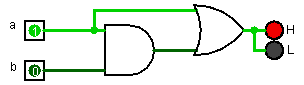
\includegraphics[width=0.5\textwidth]{2_1.png}	
	\caption{Circuit of $F_1$}
	\label{fig1}
\end{figure}

To implement the first expressions, we used a 74xx08-AND Gate and a 74xx32-OR Gate. Firstly, we implemented $a \cdot b$ which is a sub-expression of $F_1$ and we used and gate for this. Then we add  $a$ to $a \cdot b$ with or gate. As a result of this experiment,as we can see in the truth table, we found that the whole function $F_1$ depends on input a.

The truth table and circuit of $F_2$ is below.

\begin{table}[h]
    \centering
    \begin{tabular}{|c|c|c|c|c|c|}
    \hline
    a & b & $b'$ & $a + b$ & $a + b'$ & $(a + b) \cdot (a + b')$ \\ \hline
    0 & 0 & 1    & 0       & 1        & 0                  \\
    0 & 1 & 0    & 1       & 0        & 0                  \\
    1 & 0 & 1    & 1       & 1        & 1                  \\
    1 & 1 & 0    & 1       & 1        & 1                  \\ \hline
    \end{tabular}
    \caption{Truth table of $F_2$}
    \label{fig2}
\end{table}

\begin{figure}[ht]
	\centering
	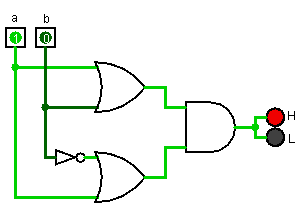
\includegraphics[width=0.5\textwidth]{2_1_2.png}	
	\caption{Circuit of $F_2$}
	\label{fig1}
\end{figure}
To implement the second expression, we used a 74xx04-Hex Inverter, a 74xx08-AND Gate and a 74xx32-OR Gate. We used the inverter to invert input $b$. Then implemented $a + b$ and $a + b'$ with or gate. Finally we merged this sub-expressions using and gate. As a result of this experiment,as we can see in the truth table, we found that the whole function $F_2$ depends on input a.

\subsection{PART 2}
In this part of experiment, logic circuit is implemented for the dual of the given theorem ($a + a \cdot b$). To determine the dual of a boolean expression AND's replace with OR's and OR's replace with AND's. Thus, we found the dual of the given theorem $a \cdot (a + b)$. We implemented the dual of given theorem for both sides using OR and AND Gates. When we compare the changes in the outputs, we saw that $a \cdot (a + b)$ is changing with input a. So we validated the truth of the theorem. \\

The circuit of the dual of the theorem is below.
\begin{figure}[ht]
	\centering
	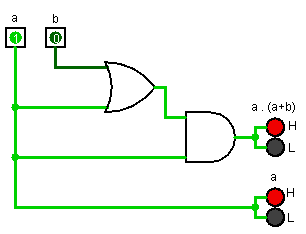
\includegraphics[width=0.5\textwidth]{2_2.png}	
	\caption{Circuit of $a \cdot (a + b)$}
	\label{fig1}
\end{figure}

\subsection{PART 3}
In the third part of the experiment, logic circuit is implemented for the complement of the given function ($F_3(a,b,c) = (a \cdot b) + (a' \cdot c)$ ). To determine the complement of a boolean expression AND's replace with OR's and OR's replace with AND's also variables replace with their inverses. When all this steps are done we found the complement of $F_3$ as $F_3'(a,b,c) = (a' + b') \cdot (a + c')$. Firstly, we inverted all inputs with 74xx04-Hex Inverter and then implemented sub-expressions $(a' + b')$ and $(a + c')$ using 74xx32-OR Gate. Finally merged the sub-circuits with 74xx08-AND Gate.\\

The circuit and truth table of the complement of given function is below.

\begin{table}[h]
\centering
\begin{tabular}{|c|c|c|c|c|c|c|c|}
\hline
a & b & c & a' & $a \cdot b$ & $a' \cdot c$ & $F_{3}$ = $a \cdot b$ + $a' \cdot c$ & $F'_{3}$ \\ \hline
0 & 0 & 0 & 1  & 0     & 0      & 0                        & 1        \\ 
0 & 0 & 1 & 1  & 0     & 1      & 1                        & 0        \\ 
0 & 1 & 0 & 1  & 0     & 0      & 0                        & 1        \\ 
0 & 1 & 1 & 1  & 0     & 1      & 1                        & 0        \\ 
1 & 0 & 0 & 0  & 0     & 0      & 0                        & 1        \\ 
1 & 0 & 1 & 0  & 0     & 0      & 0                        & 1        \\
1 & 1 & 0 & 0  & 1     & 0      & 1                        & 0        \\ 
1 & 1 & 1 & 0  & 1     & 0      & 1                        & 0        \\ \hline
\end{tabular}
\caption{Truth table for $F_3$ and it's complement}
\label{fig3}
\end{table}

\begin{figure}[ht]
	\centering
	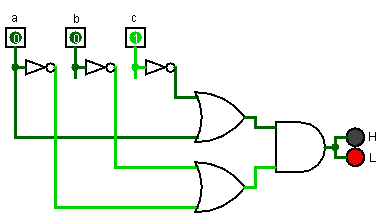
\includegraphics[width=0.5\textwidth]{2_3.png}	
	\caption{Circuit of $F_3'(a,b,c) = (a' + b') \cdot (a + c')$}
	\label{fig1}
\end{figure}

\subsection{PART 4}
In the last part of experiment, we simplified function $F_4(a,b,c,d) = U_1(1,2,5,6,9,10,13,14)$ and implemented it. We write the function in first canonical form to simplify :\\

$F_{4}(a,b,c,d) = (a'b'c'd) + (a'b'cd') + (a'bc'd) + (a'bcd') + (ab'c'd) + (ab'cd') + (abc'd) + (abc'd)$\\

To simplify the expression, we use axioms and theorems of boolean algebra :
\begin{align}
F_{4}(a,b,c,d) &= (a'b'c'd) + (a'b'cd') + (a'bc'd) + (a'bcd') + (ab'c'd) + (ab'cd') + (abc'd) + (abc'd) \notag\\ 
&= (a'b'c'd) + (a'bc'd) + (a'b'cd') + (a'bcd') + (ab'c'd) + (abc'd) + (ab'cd') + (abcd') \tag{Commutativity}\\
&= a'c'd(b' + b) + a'cd'(b'+b) + ac'd(b' + b) + acd'(b'+b) \tag{Distribution} \\
&= a'c'd(1) + a'cd'(1) + ac'd(1) + acd'(1) \tag{Inverse} \\
&= a'c'd + a'cd'+ ac'd+ acd' \tag{Identitiy} \\
&= a'c'd + ac'd + a'cd' + acd' \tag{Commutativity} \\
&= c'd(a' + a) + cd'(a' + a) \tag{Distribution} \\
&= c'd(1) + cd'(1) \tag{Inverse} \\
&= c'd + cd' \tag{Identity}
\end{align}

To implement the circuit, firstly we used 74xx04-Hex Inverter to invert inputs. Then we implemented sub-expressions $c' \cdot d$ and $c \cdot d'$ using 74xx08-AND Gate. Finally merged the sub-expressions with 74xx32-OR Gate and completed implementing the circuit. When we observed the output values of the circuit we implemented for simplified expression, we saw same outputs with truth table of $F_4$.

\begin{figure}[ht]
	\centering
	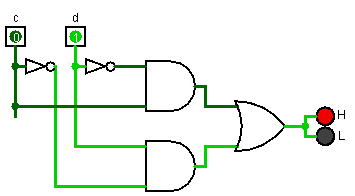
\includegraphics[width=0.5\textwidth]{2_4.png}	
	\caption{Circuit of simplified $F_4$}
	\label{fig1}
\end{figure}

\section{RESULTS}

As a result of this experiment, we learned this :
\begin{itemize}
    \item When you get the dual of both sides of an equivalence, the equivalence does not break.
    \begin{itemize}
        \item $a + a \cdot b = a$
        \item $a \cdot (a + b) = a$
    \end{itemize}
    \item How to implement XOR Gate using 74xx04-Hex Inverter, 74xx32-OR Gate and 74xx08-AND Gate.
\end{itemize}


Before the experiment, we have designed the circuits and truth tables for expressions. Throughout the experiment, we only observed the situations we planned before implementing. Because there was no factor that could cause the result to deviate.

\section{DISCUSSION}
In this experiment, we physically performed the simple expressions that we learn in Digital Circuits class. We observed the equivalence of the expressions ,that we simplified using axioms and theorems in the Digital Circuits class, with CADET and LED's. 

\section{CONCLUSION}
Since we worked a little messy at the beginning of the experiment, we did not notice a cable that we plugged in incorrectly. That's why we learned to work more carefully during the experiment. Other than that, we did not encounter any difficulties. It was a basic and interesting experiment.


\newpage
\addcontentsline{toc}{section}{\numberline {}REFERENCES}

\bibliographystyle{unsrt}
\bibliography{reference}

\end{document}

